\documentclass[journal,hidelinks]{IEEEtran}
\usepackage[utf8]{inputenc}
\usepackage[
  pdftitle={Assignment \#1},
  pdfauthor={Andrei Purcarus},
  pdfsubject={ECSE-526 -- Artificial Intelligence}
]{hyperref}
\usepackage{graphicx}
\usepackage[all]{hypcap}
\usepackage{cleveref}
\usepackage{indentfirst}
\usepackage[per-mode=symbol]{siunitx}

\title{ECSE-526 \\ Artificial Intelligence \\ Assignment \#1}
\author{Andrei~Purcarus,~260631911,~\IEEEmembership{McGill~University}}

\begin{document}
\sloppy

\maketitle

\begin{abstract}

An agent was designed to play the game of dynamic connect 4. To achieve this, adversarial search algorithms were analyzed and then improved to achieve good search performance. A heuristic evaluation function was also designed to evaluate game states when the search cannot find a clear win, and the trade-offs between heuristic complexity and search depth were analyzed. The result was a game-playing agent with adequate performance capable of playing a decent game of dynamic connect 4.

\end{abstract}

\section{Introduction}

\IEEEPARstart{T}{his} report describes the creation of an agent capable of playing the game of dynamic connect 4. First, we start by analyzing the minimax and alpha-beta search algorithms. Then, we describe a better search algorithm that we use in our agent. Finally, we analyze the heuristic evaluation functions that we use in our agent and discuss the trade-offs between the complexity of the evaluation function and the search depth achieved.

\section{Search}

We measured the performance of the minimax and alpha-beta search algorithms with depth cutoffs of $3$, $4$, $5$, and $6$ for each of the three states described in the assignment specifications. We used the heuristic described in \Cref{sec:heuristic}. For comparison, we also measured the performance of an ordered version of alpha-beta that reorders the moves at each node using the values of the heuristic function.

\subsection{Minimax}

The results for minimax search in the three different states are shown in \Cref{fig:state-1-minimax,fig:state-2-minimax,fig:state-3-minimax}. For each data set, we used a least squares fit to find an approximation of the form
\[
states = a * b^{depth}
\]
We used the exponential model since this closely approximates a tree with branching factor $b$. The resulting fits are shown on the graphs.

If we ignore the $a$ parameter since we know that its true value is $1$ ($states(0) = 1$), and we take the geometric mean of the $b$ parameters as our average branching factor, we get $b \approx 14.7$, so we have
\[
states = (14.7)^{depth}
\]

\begin{figure}[!htb]
  \centering
  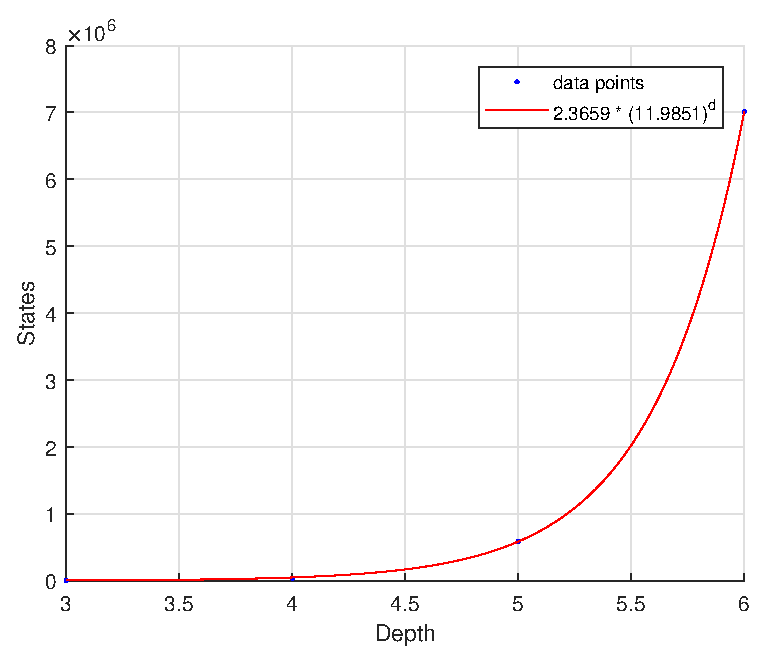
\includegraphics[width=0.6\columnwidth]{state-1/minimax.eps}
  \caption{Minimax search results for state (a).}
  \label{fig:state-1-minimax}
\end{figure}

\begin{figure}[!htb]
  \centering
  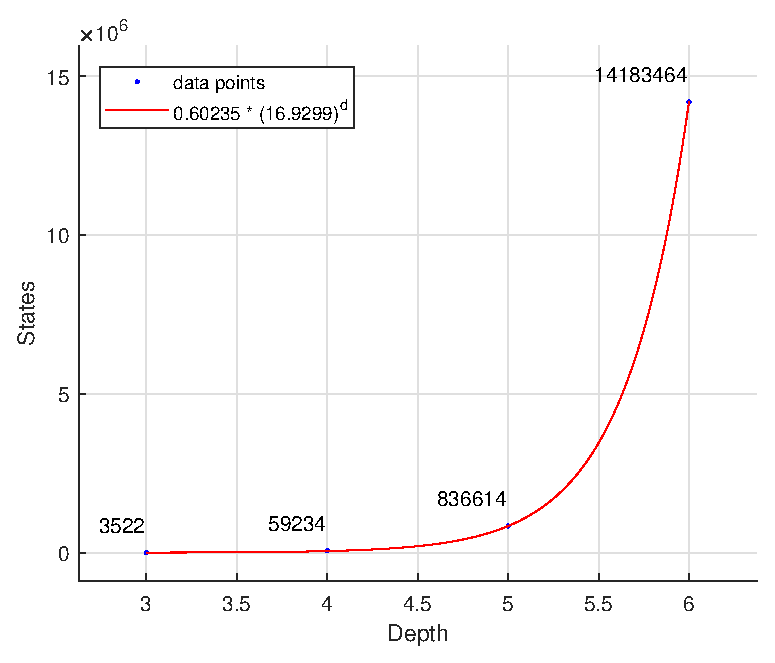
\includegraphics[width=0.6\columnwidth]{state-2/minimax.eps}
  \caption{Minimax search results for state (b).}
  \label{fig:state-2-minimax}
\end{figure}

\begin{figure}[!htb]
  \centering
  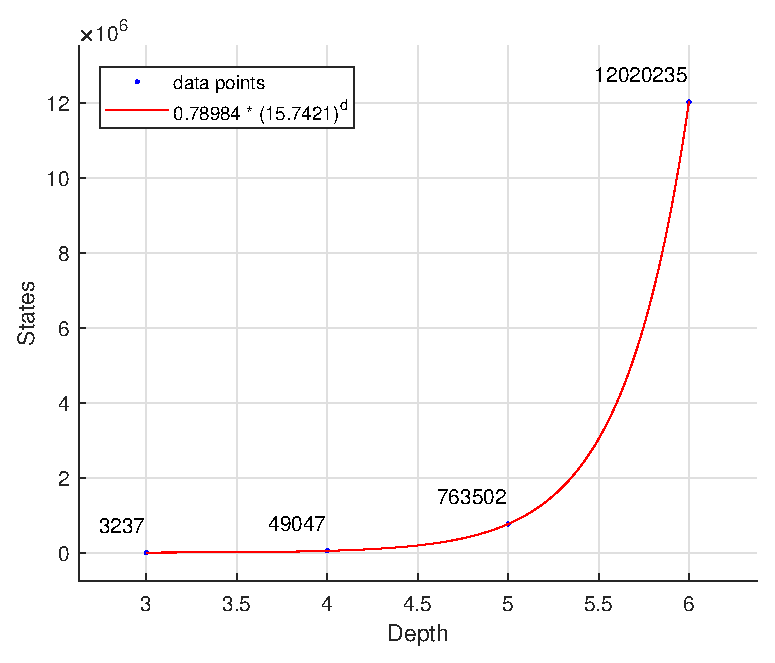
\includegraphics[width=0.6\columnwidth]{state-3/minimax.eps}
  \caption{Minimax search results for state (c).}
  \label{fig:state-3-minimax}
\end{figure}

\subsection{Alpha-Beta}

The results for alpha-beta search in the three different states are shown in \Cref{fig:state-1-alpha-beta,fig:state-2-alpha-beta,fig:state-3-alpha-beta}. For each data set, we used a least squares fit to find an approximation of the form
\[
states = a * b^{depth}
\]
We used the exponential model since this closely approximates a tree with branching factor $b$. The resulting fits are shown on the graphs.

If we ignore the $a$ parameter since we know that its true value is $1$ ($states(0) = 1$), and we take the geometric mean of the $b$ parameters as our average branching factor, we get $b \approx 5.67$, so we have
\[
states = (5.67)^{depth}
\]

\begin{figure}[!htb]
  \centering
  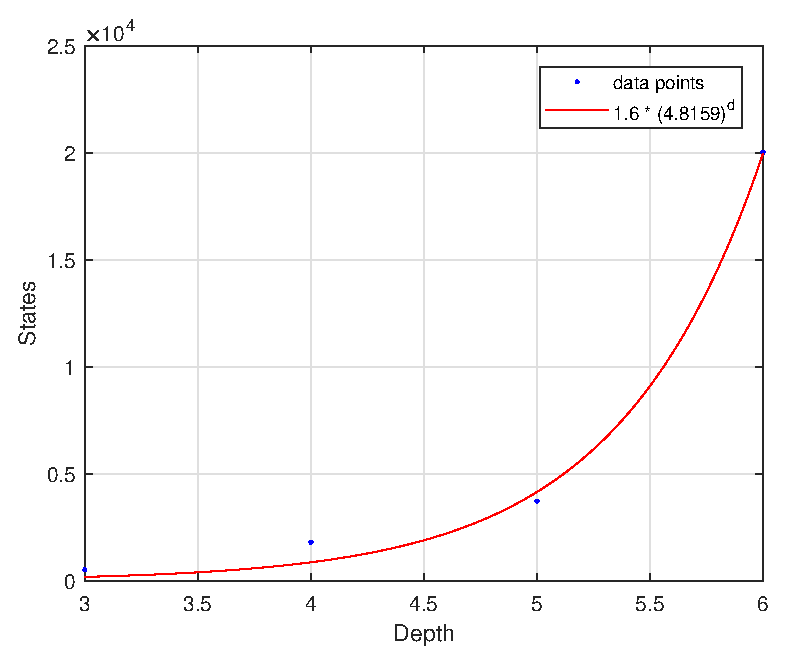
\includegraphics[width=0.6\columnwidth]{state-1/alpha-beta.eps}
  \caption{Alpha-beta search results for state (a).}
  \label{fig:state-1-alpha-beta}
\end{figure}

\begin{figure}[!htb]
  \centering
  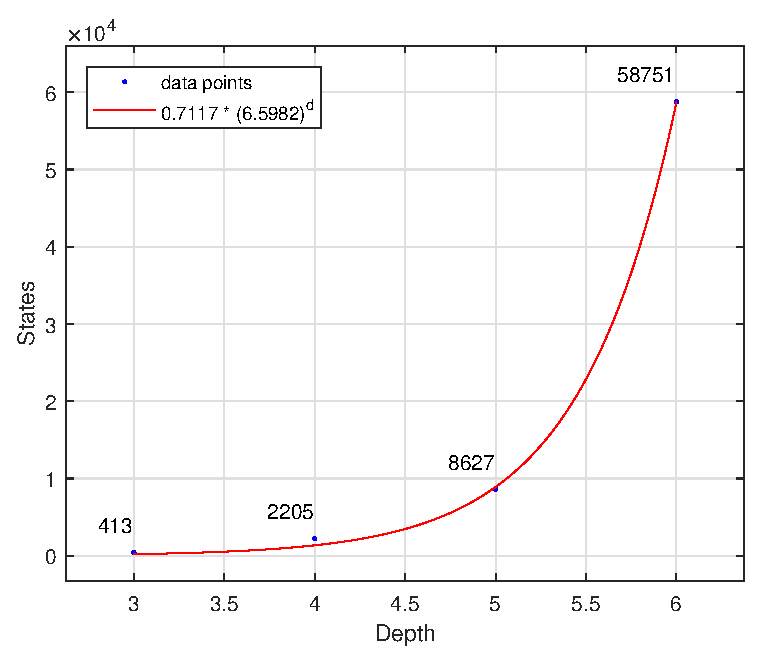
\includegraphics[width=0.6\columnwidth]{state-2/alpha-beta.eps}
  \caption{Alpha-beta search results for state (b).}
  \label{fig:state-2-alpha-beta}
\end{figure}

\begin{figure}[!htb]
  \centering
  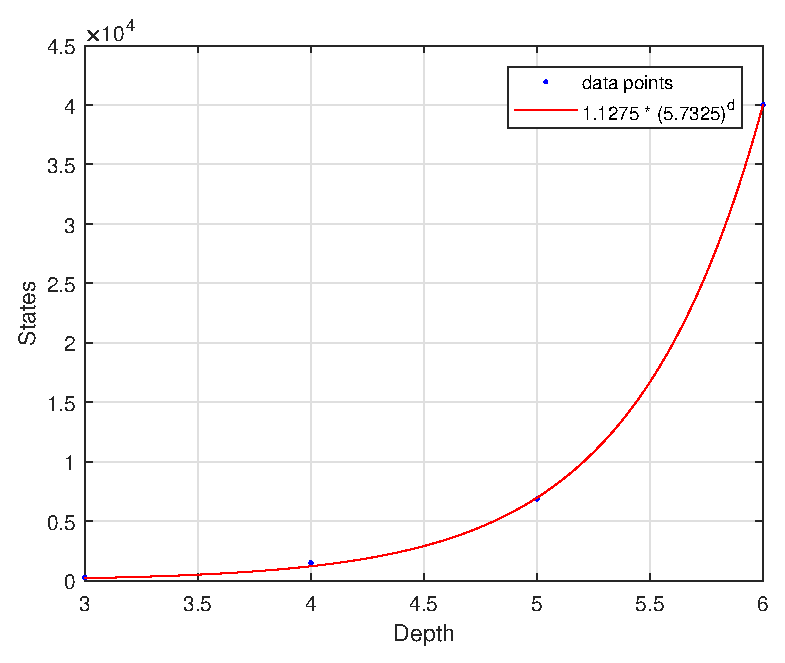
\includegraphics[width=0.6\columnwidth]{state-3/alpha-beta.eps}
  \caption{Alpha-beta search results for state (c).}
  \label{fig:state-3-alpha-beta}
\end{figure}

\subsection{Ordered Alpha-Beta}

The results for an ordered alpha-beta search in the three different states are shown in \Cref{fig:state-1-ordered-alpha-beta,fig:state-2-ordered-alpha-beta,fig:state-3-ordered-alpha-beta}. For each data set, we used a least squares fit to find an approximation of the form
\[
states = a * b^{depth}
\]
We used the exponential model since this closely approximates a tree with branching factor $b$. The resulting fits are shown on the graphs.

If we ignore the $a$ parameter since we know that its true value is $1$ ($states(0) = 1$), and we take the geometric mean of the $b$ parameters as our average branching factor, we get $b \approx 3.0$, so we have
\[
states = (3.0)^{depth}
\]

Note that the $a$ parameter for this type of search deviates from the ideal. This is due to the fact that the least squares fit was not as good as for the other two types of search. A larger sample size would be needed to get a better approximation.

\begin{figure}[!htb]
  \centering
  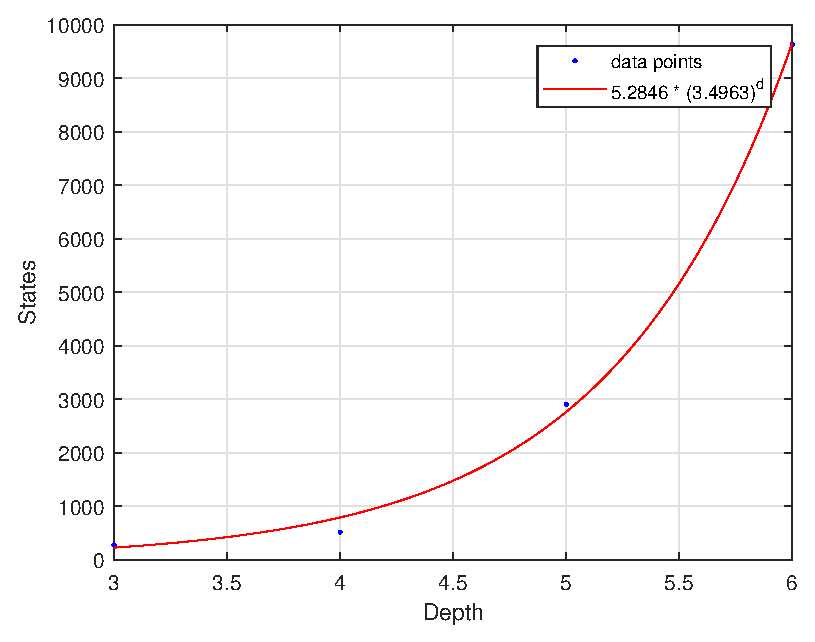
\includegraphics[width=0.6\columnwidth]{state-1/ordered-alpha-beta.eps}
  \caption{Ordered alpha-beta search results for state (a).}
  \label{fig:state-1-ordered-alpha-beta}
\end{figure}

\begin{figure}[!htb]
  \centering
  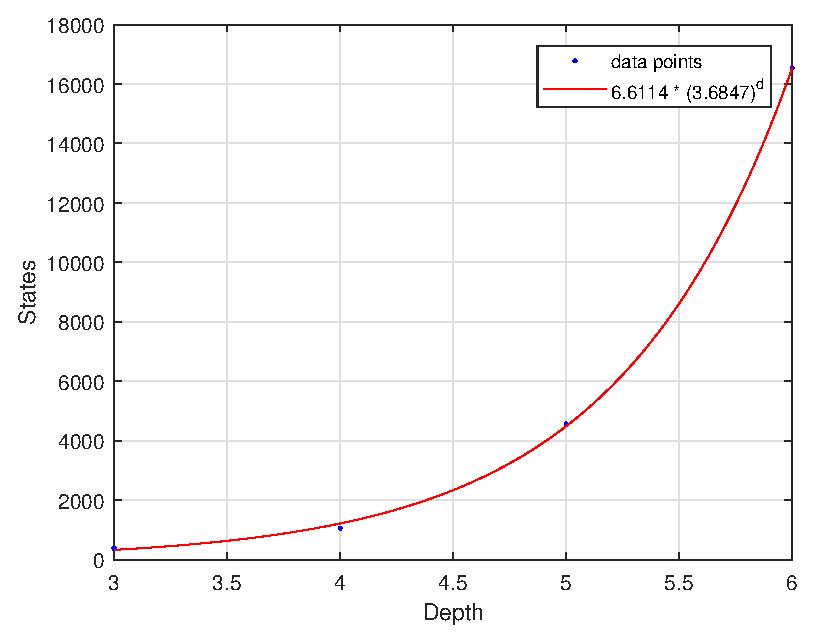
\includegraphics[width=0.6\columnwidth]{state-2/ordered-alpha-beta.eps}
  \caption{Ordered alpha-beta search results for state (b).}
  \label{fig:state-2-ordered-alpha-beta}
\end{figure}

\begin{figure}[!htb]
  \centering
  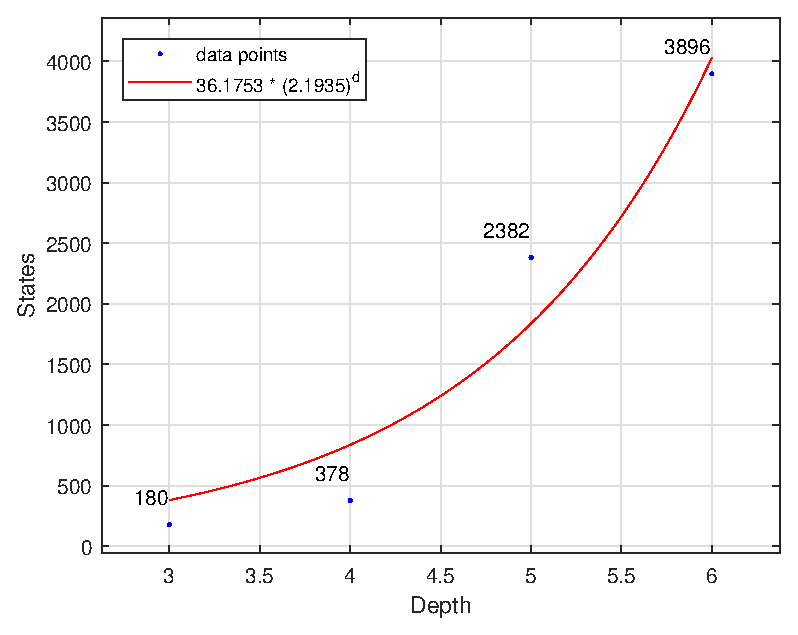
\includegraphics[width=0.6\columnwidth]{state-3/ordered-alpha-beta.eps}
  \caption{Ordered alpha-beta search results for state (c).}
  \label{fig:state-3-ordered-alpha-beta}
\end{figure}

\subsection{Comparison}

Comparing the results obtained, we can see that alpha-beta pruning has a significant performance advantage over minimax, with an average branching factor $2.6$ times smaller. We can also see that move ordering using the heuristic function further diminishes this branching factor.

In theory, alpha-beta search can reach an effective branching factor as low as $\sqrt{b_{minimax}} = 3.83$. This occurs when all the moves are ordered perfectly according to their real values. We can see that in this case, move ordering using the heuristic function actually exceeded this theoretical limit. This can be accounted for by our limited sample size, which makes it hard to get a good least squares fit and thus has some error in the measure of the effective branching factor.

\section{Better Search}

In order to make the agent competitive, we used an augmented version of alpha-beta search. The first concern was the time limit imposed by competition. In order to be able to use a maximal amount of search time, we used an iterative version that increments the search depth until it runs out of time. To take advantage of the results of past depths in the next search, we sort the actions at the root after each iteration based on the values found. It is important that the sort be stable, since this ensures that an action that was more favorable at a lower depth will still be ahead of other actions that became equal at a higher depth. In this way, the best action across all depths searched is chosen.

In addition, the moves at nodes other than the root are ordered by the heuristic function before being searched. This yields better alpha-beta pruning performance. The exception is those nodes at the bottom of the tree for which the cost of sorting outweighs the benefit. A basic analysis shows that this cost is
approximately $h*b + c*b*lg(b)$ and the savings are at most $h*b^{\left \lfloor{d/2}\right \rfloor}$, where $b$ is the actual branching factor, $d$ is the distance between the node and the leaves of the tree, $h$ is the cost of a heuristic evaluation, and $c$ is the cost of a comparison and swap for sorting. This gives $d \ge 4$.

Next, a transposition table was added to keep track of states we've already seen. In order to limit the memory usage, the size was limited to $4$ million elements, and a LRU replacement strategy was used to replace old states.

Finally, to take advantage of all the time we have available, we also modified the agent to perform search on the opponent's turn. The results of this search are ignored, but the fact that search is performed allows the transposition table to be updated, which speeds up search on our turn.

For the complete implementation, see the \textbf{IterativeAlphaBeta} class in the \textit{src/search/iterative-alpha-beta.h} file.

\section{Heuristics}
\label{sec:heuristic}

To create heuristics, we used the guiding principle that a heuristic function should lead the agent to a position where it can find a winning position within its search depth. Two simple heuristics were combined to achieve this goal. These heuristics award points to connected pieces and to a dominant central position.

\subsection{Connected Pieces}

This heuristic awards $n(n-1)/2$ points for a set of $n$ connected pieces. This is important since the goal of the game is to get $4$ pieces in a row, so rewarding partial completion of the goal is likely to lead us to the goal. The corresponding class is \textbf{ConnectedPiecesV1}, which corresponds to one of the versions of this heuristic. For the other versions considered, see the \textit{src/game/heuristics/connected-pieces.h} file.

\subsection{Central Dominance}

This heuristic awards a certain number of points to each piece based on its position on the board (see \Cref{tab:central-dominance}), with central pieces getting more points. The values were chosen to give an approximate $1$ point increase as the pieces move to a more central square, with slight deviations to favor more central positions within a square. The values were also chosen to be exactly representable in binary floating point to avoid round-off errors. This heuristic gives the agent the incentive to move pieces to the center of the board, which in turn is apt to provide more opportunities for both connecting pieces or stopping the opponent from connecting pieces. In addition, this heuristic awards bonus points in the form of a multiplicative factor for a player that has at least $3$ pieces in the central positions (corresponding to the non-zero values in \Cref{tab:central-dominance}). The corresponding class is \textbf{CentralDominanceV2}, which corresponds to one of the versions of this heuristic. For the other versions considered, see the \textit{src/game/heuristics/central-dominance.h} file.

\begin{table}[!htb]
	\centering
	\caption{Central Dominance Lookup Table.}
	\label{tab:central-dominance}
	\resizebox{\columnwidth}{!}{\begin{tabular}{c|ccccccc}
		  &    1    &    2    &    3    &    4    &    5    &    6    &    7    \\ \hline
		1 & 0.0000f & 0.0000f & 0.0000f & 0.0000f & 0.0000f & 0.0000f & 0.0000f \\
		2 & 0.0000f & 0.8125f & 1.0000f & 1.1875f & 1.0000f & 0.8125f & 0.0000f \\
		3 & 0.0000f & 1.0000f & 2.0000f & 2.1875f & 2.0000f & 1.0000f & 0.0000f \\
		4 & 0.0000f & 1.1875f & 2.1875f & 2.3750f & 2.1875f & 1.1875f & 0.0000f \\
		5 & 0.0000f & 1.0000f & 2.0000f & 2.1875f & 2.0000f & 1.0000f & 0.0000f \\
		6 & 0.0000f & 0.8125f & 1.0000f & 1.1875f & 1.0000f & 0.8125f & 0.0000f \\
		7 & 0.0000f & 0.0000f & 0.0000f & 0.0000f & 0.0000f & 0.0000f & 0.0000f
	\end{tabular}}
\end{table}

\subsection{Complexity Trade-offs}

The use of a more complex evaluation function, provided this function more accurately evaluates a game state, is to be favored over a simpler one. There are several reasons for this. First, since the time taken by the search algorithm is exponential in depth and linear in evaluation function complexity, the loss of depth from having a more complex evaluation function is not likely to be significant. For example, if the evaluation function doubles in computation time and the average branching factor is $3.0$, at most the search will lose a depth of one. Second, a shallower search will use up less memory than a deeper one, though this is not as significant a concern since the memory usage for depth-first search is linear in depth. Third, a more complex evaluation function that better represents the game state is likely to lead to a better position and therefore has a better chance of winning, despite having a slightly lower search depth.

To test this trade-off, we played an agent using both \textbf{ConnectedPiecesV1} and \textbf{CentralDominanceV2} against an agent using only \textbf{ConnectedPiecesV1}. Both agents used the \textbf{IterativeAlphaBeta} search with a time limit of $\SI{1}{\second}$. To get an estimate of the speed of these agents, we ran them both on state (b) from the assignment specifications for $4$ runs and averaged the results. Agent 1 managed a depth of $10$, with $1,002,806$ states evaluated. Agent 2 managed a depth of $11$, with $1,363,925$ states evaluated. Agent 2 is therefore $\SI{36}{\percent}$ faster, and can reach an extra level of depth. However, after playing $20$ games between them, $10$ for each color, the results were $9$ wins and $1$ draw for agent 1 when it was playing as white and $9$ wins and $1$ draw when it was playing as black. Clearly, the more complicated heuristic dominated the simpler one, despite the search disadvantage. Note that a draw is defined as a repetition of moves, which indicated that the agents have reached a stalemate.

\section{Conclusions}

In conclusion, a game-playing agent was designed and analyzed. The basic alpha-beta search algorithm was augmented with several improvements, and a decent heuristic was designed for evaluating game states. The result is an agent that performs adequately in playing the game of dynamic connect 4.

\section{Acknowledgements}

High-level strategy and heuristics were discussed with Andrew Lowther and Sean Stappas.

\bibliographystyle{IEEEtran}
\bibliography{IEEEabrv,references}

\end{document}
